\documentclass[]{article}
\usepackage{lmodern}
\usepackage{amssymb,amsmath}
\usepackage{ifxetex,ifluatex}
\usepackage{fixltx2e} % provides \textsubscript
\ifnum 0\ifxetex 1\fi\ifluatex 1\fi=0 % if pdftex
  \usepackage[T1]{fontenc}
  \usepackage[utf8]{inputenc}
\else % if luatex or xelatex
  \ifxetex
    \usepackage{mathspec}
  \else
    \usepackage{fontspec}
  \fi
  \defaultfontfeatures{Ligatures=TeX,Scale=MatchLowercase}
\fi
% use upquote if available, for straight quotes in verbatim environments
\IfFileExists{upquote.sty}{\usepackage{upquote}}{}
% use microtype if available
\IfFileExists{microtype.sty}{%
\usepackage{microtype}
\UseMicrotypeSet[protrusion]{basicmath} % disable protrusion for tt fonts
}{}
\usepackage[margin=1in]{geometry}
\usepackage{hyperref}
\hypersetup{unicode=true,
            pdfauthor={Daniel Kaplan},
            pdfborder={0 0 0},
            breaklinks=true}
\urlstyle{same}  % don't use monospace font for urls
\usepackage{graphicx,grffile}
\makeatletter
\def\maxwidth{\ifdim\Gin@nat@width>\linewidth\linewidth\else\Gin@nat@width\fi}
\def\maxheight{\ifdim\Gin@nat@height>\textheight\textheight\else\Gin@nat@height\fi}
\makeatother
% Scale images if necessary, so that they will not overflow the page
% margins by default, and it is still possible to overwrite the defaults
% using explicit options in \includegraphics[width, height, ...]{}
\setkeys{Gin}{width=\maxwidth,height=\maxheight,keepaspectratio}
\IfFileExists{parskip.sty}{%
\usepackage{parskip}
}{% else
\setlength{\parindent}{0pt}
\setlength{\parskip}{6pt plus 2pt minus 1pt}
}
\setlength{\emergencystretch}{3em}  % prevent overfull lines
\providecommand{\tightlist}{%
  \setlength{\itemsep}{0pt}\setlength{\parskip}{0pt}}
\setcounter{secnumdepth}{0}
% Redefines (sub)paragraphs to behave more like sections
\ifx\paragraph\undefined\else
\let\oldparagraph\paragraph
\renewcommand{\paragraph}[1]{\oldparagraph{#1}\mbox{}}
\fi
\ifx\subparagraph\undefined\else
\let\oldsubparagraph\subparagraph
\renewcommand{\subparagraph}[1]{\oldsubparagraph{#1}\mbox{}}
\fi

%%% Use protect on footnotes to avoid problems with footnotes in titles
\let\rmarkdownfootnote\footnote%
\def\footnote{\protect\rmarkdownfootnote}

%%% Change title format to be more compact
\usepackage{titling}

% Create subtitle command for use in maketitle
\newcommand{\subtitle}[1]{
  \posttitle{
    \begin{center}\large#1\end{center}
    }
}

\setlength{\droptitle}{-2em}

  \title{}
    \pretitle{\vspace{\droptitle}}
  \posttitle{}
    \author{Daniel Kaplan}
    \preauthor{\centering\large\emph}
  \postauthor{\par}
      \predate{\centering\large\emph}
  \postdate{\par}
    \date{2018-12-19}


\begin{document}

(ref:beech-run-mug) Exercise in file beech-run-mug

TITLE GOES HERE: @ref(fish-dive-plant) involved a comparison between
hybrid and non-hybrid cars.

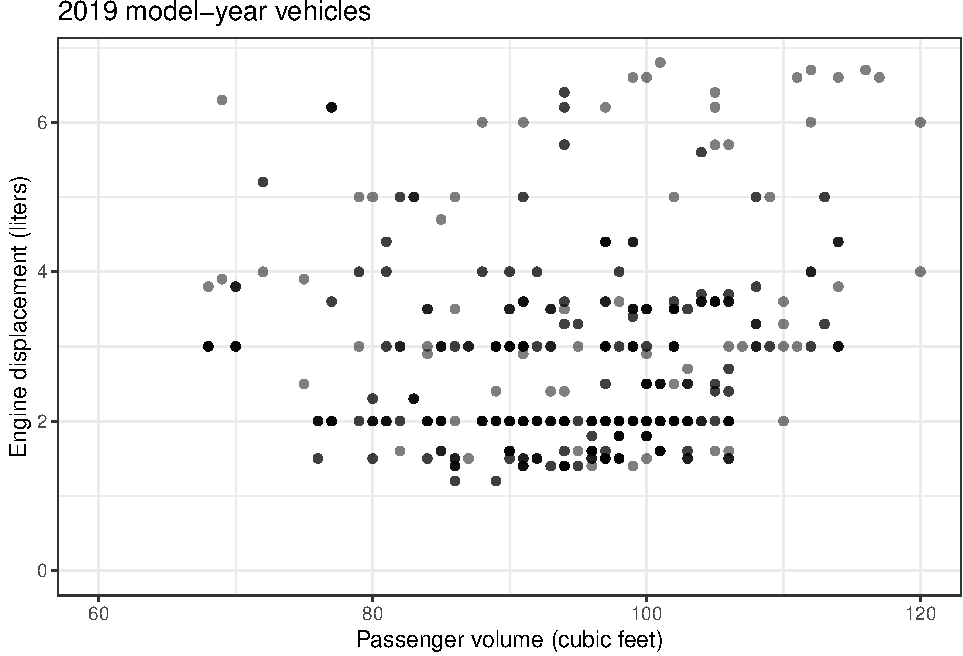
\includegraphics[width=0.8\linewidth]{beech-run-mug_files/figure-latex/beech-run-mug-1-1}

\begin{enumerate}
\def\labelenumi{\arabic{enumi}.}
\tightlist
\item
  Divide the horizontal axis into, strata: \textless{}70, 70 to 80, 80
  to 90, and so on.

  \begin{enumerate}
  \def\labelenumii{\alph{enumii}.}
  \tightlist
  \item
    What is a prediction interval on displacement for the 70 to 80
    category?
  \item
    What is a prediction interval on displacement for the 100 to 110
    category?
  \end{enumerate}
\end{enumerate}

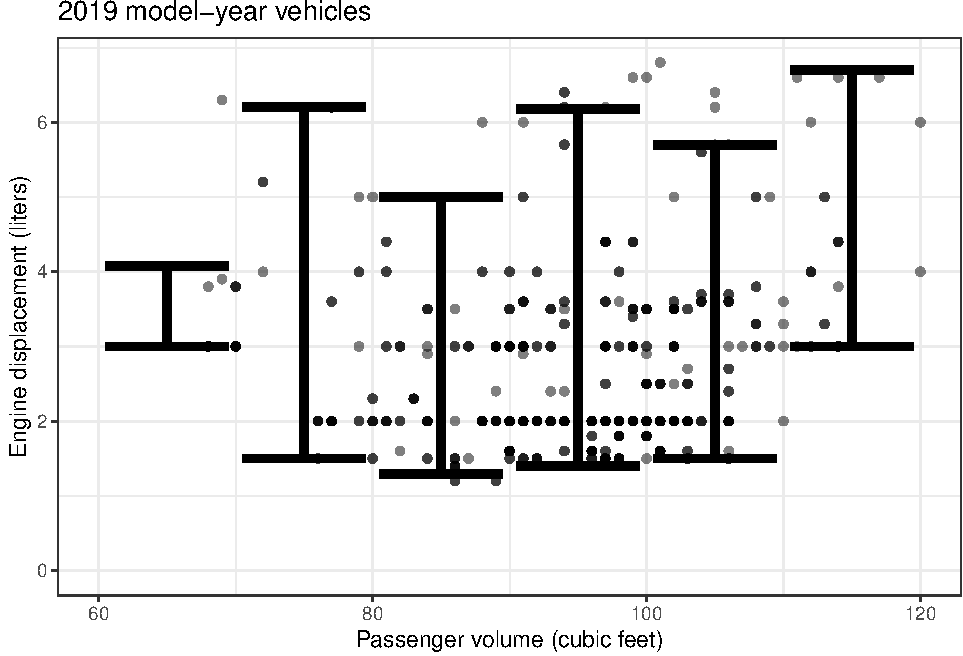
\includegraphics[width=0.8\linewidth]{beech-run-mug_files/figure-latex/beech-run-mug-2-1}

\begin{enumerate}
\def\labelenumi{\arabic{enumi}.}
\setcounter{enumi}{1}
\tightlist
\item
  Comparing the 70 to 80 and the 100 to 110 cubic feet strata:

  \begin{enumerate}
  \def\labelenumii{\alph{enumii}.}
  \tightlist
  \item
    how does the engine displacement vary? -A- The prediction intervals
    are practically identical.
  \item
    Is there a strong relationship between passenger volume and engine
    displacement? -A- Since the prediction intervals don't vary,
    passenger volume doesn't seem to be related to displacement.
  \end{enumerate}
\end{enumerate}

\begin{quotation}\em

OK. This is the answer text.

This is a block of answer text. This is a block of answer text.

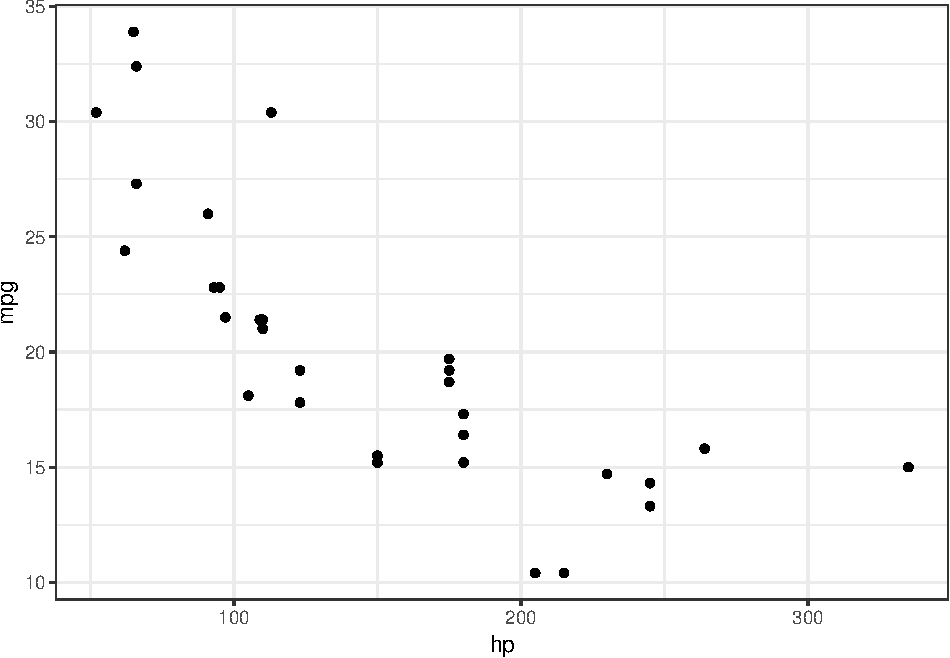
\includegraphics[width=0.8\linewidth]{beech-run-mug_files/figure-latex/unnamed-chunk-1-1}
\end{quotation}

\begin{enumerate}
\def\labelenumi{\arabic{enumi}.}
\setcounter{enumi}{2}
\tightlist
\item
  Consider the vehicles at the extremes of passenger volume, either very
  small (\textless{} 70) or very large (\textgreater{} 110).

  \begin{enumerate}
  \def\labelenumii{\alph{enumii}.}
  \tightlist
  \item
    Are these extreme vehicles systematically different in displacement
    than the large majority of vehicles with passenger volumes between
    70 and 110 cubic feet? -A- Yes. Both very small and very large
    passenger-volume vehicles tend to have higher displacements than the
    vehicles in the middle.
  \item
    Are the very large and very small vehicles similar or different from
    each other in terms of displacement? Give a common-sense explanation
    for the pattern. -A- Both the very small and the very large
    passenger-volume vehicles are built for special purposes. The very
    small vehicles are sports cars, which demand a high engine power and
    therefore high displacement. The very large vehicles are meant to
    carry large cargos or tow large loads. This also demands relatively
    high engine power.
  \end{enumerate}
\end{enumerate}


\end{document}
